\chapter{Adversarial Examples Taxonomy}

This chapter focuses on Adversarial Crafting and how these examples can be used to exploit some of the Deep Neural Networks caveats seen in the last chapter. Firstly the Fast Gradient Sign method will be explained along with some results. Secondly, a brief discussion on the empty pockets of space created by neural networks allow such technique to create adversarial. Finally a discussion of the potential threats these pose to systems relying on machine learning algorithms to perform their tasks.


\section{Foundations}

Understanding of why adversarial samples can exist requires exploration of how learning models are built. The training data is a corpus of samples taken from a expected input distribution and are labeled accordingly to their desired class. For instance, this sample data would be a large number of emails or a huge data set of images. The labels are then taken as ground truth when constructing models to be used at runtime.

The integrity of deep learning systems usually is that of that measures how accurate the system is when performing a classification task. This metric is of paramount importance and, therefore, should be a common target for techniques trying to exploit such algorithms vulnerabilities. Specifically, an adversary of a deep learning system seeks to provide an input X' that results in incorrect output classification. The incorrectness of the prediction can be represented into different natures and can impact the classifier output in different ways.

Adversary drivers could be explained into four goals as discussed by Papernot(2016) \cite{papernot_thesis_2016}. Confidence reduction is the adversary potential to introduce class ambiguity by reducing classification confidence. Misclassification happens when a label of the model being previously correct is changed to an incorrect output label. On the same way, one could use a Targeted misclassification to produce inputs that forces outputs into a specific label. Finally, the source/target misclassification forces the output classification of a specific input to be a specific target class.

\section{Domain Shift}

Regardless of the technique, a machine learning model represents an approximation of the phenomena being modeled. In most cases the training data is unable to represent all possible input feature vectors and, therefore, can not full capture a complete understanding of the target domain. A problem arises when input examples are able to exploit the system by providing samples that are not within the aforementioned input domain. They usually use information about the system to find where the model is inaccurate owing to missing items of the given training set.

Classification accuracy should be carefully measured when training a model. For instance, the value of the training set is usually higher than the one on the test set. This happens when the samples of the training can not cover the entire data distribution space and therefore the domain covered differs from the one on the test set. A poor performance on the test set means that the divergence of both distributions (training and test domains) is high. 

What adversaries do is to force the domain shift in a way that the model is unable to generalize well on test data. Since data in almost circumstances can not cover the entire feature space, the real decision boundary of a classification model generally becomes more complex as the phenomenon becomes more nuanced and the feature and dimension space becomes larger. This complexity is exploited by adversaries through the use of the model error as a guideline for perturbing a sample.

\begin{figure}[!h]
\centering
	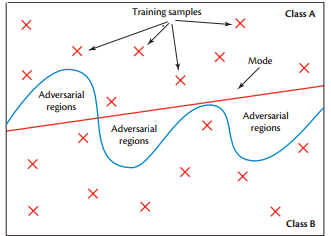
\includegraphics[scale=1.0]{adv_space.png}
\caption{Two Dimensional Representation of unexplored adversarial regions \cite{papernot_2017}}
\label{fig:adv_space}
\end{figure}

\section{Fast Gradient Sign}

The Fast Gradient Signed method developed by Goodfellow et al. (2014) has been used as the foundation of many of the experiments in adversarial crafting. The results have led to the hypothesis that DNNs can possibly have linear behavior when in very high dimensional space.  Most inputs were miss-classified not only on Goodfellow et. al \cite{goodfellow2014}  experiments but many other. This shows that adversarial examples are not hard to find. The method consists on using gradient information to generate image noises that changes classification outputs.

$$ C(x + \delta)\approx C(x) + \delta * \nabla C$$

The equation aims into adding noise that emphasizes the pixels in the image with the highest importance, so the resulting perturbation can likely lead to a misclassified result. By using the \textit(sign) function of the gradient, it is assured that the value will grow linearly with the number of the dimensions \cite{goodfellow2014}. The result of many small pixel changes is likely to generate an image with a wrong label in the network output.

$$ C(x + \delta)\approx C(x) + \delta * sign(\nabla C)$$

Billovits et al (2016) categorized four different categories of adversarials generated by FGSM. True Adversarial are those given a completely different label after being perturbed. Re-Focused adversarial is the method that changes the focus of an image by giving a classification of an object that used to have lower significance while keeping the original object presence. Conaturally Adversarial are those where the new output has some close relation to the miss-classified result (e.g. Dog and Cat). Finally, Benign adversarial hapeens when neural networks misses the top prediction of the original image but the adversarial example gets classified correctly with high confidence \cite{billovits}.

\begin{figure}[!h]
\centering
	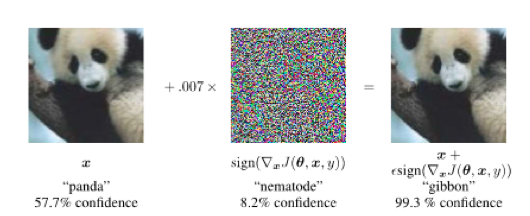
\includegraphics[scale=0.6]{panda.png}
\caption{Adversarial example crafting with fast gradient sign \cite{goodfellow2014}.}
\label{fig:fgsm_craft}
\end{figure}

\section{Unrecognizable Images}\label{subsec:unrec}

Adversaries, on the other hand, are not only comprised of small perturbations on known images. Nguyen et al (2015) presented a method for producing images that are unrecognizable to humans, but are nonetheless labeled as recognizable objects by DNNs \cite{nguyen2015}. For instance, a DNN would classify a noise-filled image crafted using their technique with high confidence. These images were named $fooling images$ since they do not have a source class but are crafted solely to perform a targeted misclassification attack.

\begin{figure}[!h]
\centering
	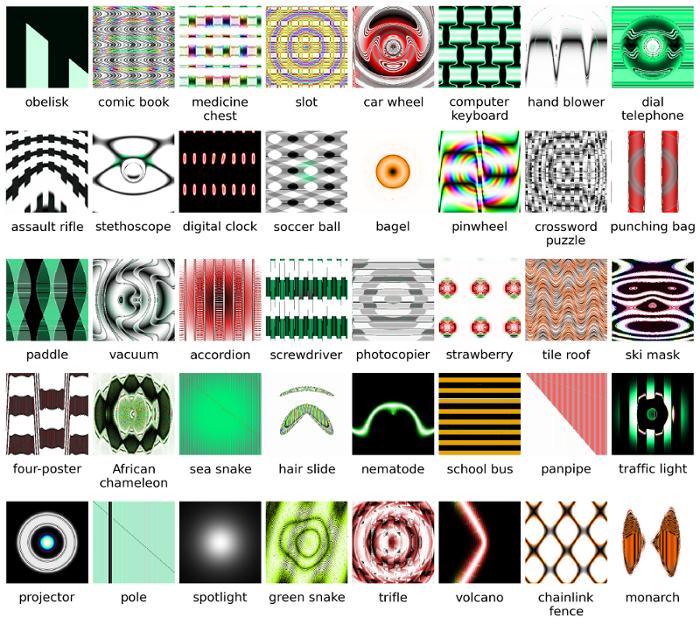
\includegraphics[scale=1.]{unrec_images.png}
\caption{Examples of noisy images classified with high confidence \cite{nguyen2015}.}
\label{fig:unrec_images}
\end{figure}


\section{Adversarials in the Physical World}\label{sec:physical}

All the aforementioned techniques were based into feeding information directly into machine learning systems. Such model only takes into consideration situations in which attacks take place entirely within the computer. For instance, these techniques could be used by attackers to avoid spam filters or malware detectors. Even though the study is utterly relevant, a recent study conducted by \cite{goodfellow2016} have shown that it is possible to craft adversarial samples in order to perform attacks on machine learning systems which are operating in the physical world.

Although the Fast Gradient Sign method have been successful on crafting adversarial examples, there are some extensions of the method that can be used in order to create perturbations that are more likely to work in the physical world. Firstly, \cite{goodfellow2016} introduced a variation named \textit{Basic Iterative Method}. This technique consists of applying the fast method multiple times with small step sizes and making sure that all pixels are within a $\epsilon$-neighbourhood of the original image. The number of iterations was chosen heuristically with goals of being sufficient enough to have the adversarial example reaching the edge of the $\epsilon$ max-norm.

In order to perform experiments, clean photos of adversarial examples created using the three methods were taken and fed into a machine learning system using Deep Convolutional Neural Networks (Inception V3). Adversarial Images created using the "fast" method were more robust when compared to the iterative methods. The hypothesis behind the result is that iterative methods create more subtle perturbations that can be easily be destroyed by the photo transformation process (Photo Printing as described above). Overall, it could be expected that about 2/3 of the images would be top-1 misclassified and about 1/3 top-5 misclassified by the fast method using an $\epsilon$ of 16.

Adversarial examples is not only feasible on digital attacks but also on physical world scenarios. By using the correct perturbation algorithm with optimized hyperparameters one can use printed digital photos to fool day-to-day machine learning systems. As more and more machine learning is becoming part of our environment, techniques for avoiding such attacks need to be developed so these systems can become less vulnerable to any kind of attack.